\documentclass[11pt, letter]{amsart}


\usepackage[margin=1in]{geometry}
\usepackage{amsthm}
\usepackage{amsmath}
\usepackage{amssymb}
\usepackage{enumerate}
\usepackage[inline]{enumitem}
\usepackage{graphicx}

\newtheorem*{theorem*}{Theorem}
\newtheorem*{lemma*}{Lemma}
\theoremstyle{definition}
\newtheorem{problem}{Problem}[]
\newtheorem{exercise}{Exercise}[]
\newtheorem*{definition*}{Definition}

\newcommand\cF{{\mathcal F}}

\title[Math 4032: Homework \#2\qquad Due February 3 at 1:59pm]{Math 4032: Homework \#2\\
  Due February 3 at 1:59pm}


\begin{document}


\maketitle


\begin{center}
  \textit{You are strongly encouraged to typeset your homework solutions using \LaTeX.}
\end{center}

\vspace{1cm}
The relevant background material for this assignment is covered in Chapters 3.4--3.8 and 7 of the Matou\v{s}ek--Ne\v{s}et\v{r}il book.

\vspace{1cm}
The following problems are optional exercises not to be turned in.  Problems to be turned in for a grade begin on the next page.  

\begin{exercise}
  In class we proved that $\binom{n}{k} \leq (en / k)^k$ for every $n \in \mathbb N$ and $k \in [n]$.  Provide alternative proofs
  \begin{enumerate}
  \item using induction on $k$ and
  \item algebraically, using the bounds $e(n / e)^n \leq n! \leq en (n / e)^n$.
  \end{enumerate}
\end{exercise}

\begin{exercise}
  Using Stirling's formula, prove that $\binom{2m}{m} \sim 2^{2m} / \sqrt{\pi m}$.
\end{exercise}

\begin{exercise}
  Use the Inclusion-Exclusion Principle to count the number of numbers less than $100$ that are not divisible by a square of any integer greater than 1.
\end{exercise}

\begin{exercise}
  Recall that $D(n)$ is the number of derangements of an $n$-element set.  Prove that the number of permutations of an $n$-element set with exactly $k$ fixed points is $\binom{n}{k} D(n - k)$.
\end{exercise}

\begin{exercise}
  Prove that
  \begin{equation*}
    D(n) = n! - \sum_{k=1}^n \binom{n}{k}D(n - k).
  \end{equation*}
\end{exercise}

\clearpage
  Recall that the $n$th harmonic number is $H_n = \sum_{i=1}^n 1 / i$.
\begin{problem}
  Prove that
  \begin{equation*}
    \ln n < H_n \leq 1 + \ln n
  \end{equation*}
  for every $n \in \mathbb N$.
  \textit{Hint: Use induction on $n$.  Use the fact that $e^x > 1 + x$ to prove that $\ln n + 1 / n < \ln (n + 1)$.}
\end{problem}

\begin{proof}
Let $H_n = \sum_{i = 1}^n \frac{1}{i}$ as is defined above. Consider then,
\begin{align*}
    \ln(n) &= \int_1^n\frac{1}{x}dx\\
    &= \sum_{i = 1}^{n - 1}\int_i^{i + 1}\frac{1}{x}dx\\
    &\leq \sum_{i = 1}^{n - 1}\int_i^{i + 1}\frac{1}{i}dx\\
    &= H_{n - 1}\\
    &< H_n.
\end{align*} Similarly, we then have that 
\begin{align*}
    \ln(n) &= \int_1^n\frac{1}{x}dx\\
    &= \sum_{i = 1}^{n - 1}\int_i^{i + 1}\frac{1}{x}dx\\
    &\geq \sum_{i = 1}^{n - 1}\int_i^{i + 1}\frac{1}{i + 1}dx\\
    &= H_n - 1.
\end{align*} This then implies that
\begin{equation*}
    \ln(n) < H_n \leq 1 + \ln(n)
\end{equation*}
as desired.
\end{proof}

\clearpage
Recall that $\pi(n)$ is the number of primes in the set $[n]$.  In class, we proved $\pi(n) = O(n / \ln n)$.  In the following problem, you will prove $\pi(n) = \Omega(n / \ln n)$, which completes the proof of the ``Weak Prime Number Theorem''.

For $n \in \mathbb N$ and a prime $p$, let $\nu_p(n)$ denote the largest integer $k$ such that $p^k \mid n$.  Equivalently, $\nu_p(n)$ is the exponent to which $p$ appears in the prime factorization of $n$.    

\begin{problem}
Prove the following, and conclude that $\pi(n) = \Omega(n / \ln n)$.
  \begin{enumerate}[label={(\alph*)}]
  \item Prove that every prime $p$ and every $n \in \mathbb N$ satisfies
    \begin{equation*}
      \nu_p(n!) = \sum_{k=1}^\infty \left\lfloor \frac{n}{p^k}\right\rfloor.
    \end{equation*}
    \begin{proof}
        Let assumptions be as in the problem statement, given that $\nu_p(n)$ denotes the largest $k$ such that $p^k$ divides $n$. By the definition $n!$ is the product of $\{1, 2, ..., n\}$ so we know we will have at least one factor of $p$ in $n!$ for each multiple of $p$ in $\{1, 2, ..., n\}$ and there will be $\lfloor \frac{n}{p} \rfloor$ is a multiple of $p$. Similarly, we will have a factor of $p^2$ which will contribute an additional factor of $p$ and then $\lfloor \frac{n}{p^2}\rfloor$ will be a multiple of $p^2$ in the set $\{1, 2, ..., n\}$ and so on. Now, let's say that $k$ is the largest factor of $p$ such that $p^k \mid n!$. Then we know for $j > k$ that $p^j$ will not divide any $\{1, 2, ..., n\}$ implying that $p^j > n \forall j > k$ further implying that $\lfloor \frac{n}{p^j} \rfloor = 0 \forall j > k$. Thus, we have that $\nu_p(n!) = \lfloor \frac{n}{p} \rfloor + \lfloor \frac{n}{p^2} \rfloor + ... + \lfloor \frac{n}{p^k} \rfloor + 0 + 0 ... \Rightarrow \nu_p(n!) = \sum_{w = 1}^k \lfloor \frac{n}{p^w} \rfloor + \sum_{\zeta > k} \lfloor \frac{n}{p^\zeta} \rfloor \Rightarrow \nu_p(n!) = \sum_{k = 1}^\infty \lfloor \frac{n}{p^k} \rfloor$ as desired.
    \end{proof}
  \item Using (a), prove that every prime $p$ and every $n \in \mathbb N$ satisfies
    \begin{equation*}
      \nu_p\left(\binom{2n}{n}\right) = \sum_{k=1}^\infty\left(\left\lfloor\frac{2n}{p^k}\right\rfloor  - 2\left\lfloor \frac{n}{p^k}\right\rfloor \right)
    \end{equation*}
    \textit{Hint: Use that $\binom{2n}{n} = (2n)! / (n!)^2$.}
    \begin{proof}
        We know that $\binom{2n}{n} = \frac{(2n)!}{(n!)^2}$. By definition of $\nu_p(n)$ we know that $p^k \mid n$. Then we have that $\nu_p(\binom{2n}{n}) = \nu_p(\frac{(2n)!}{n!^2}) = \nu_p((2n)!) - \nu_p((n!))^2 = \nu_p((2n)!) - (\nu_p(n!) + \nu_p(n!)).$ Also note, $\nu_p((n!)^2) = \nu_p(n!) + \nu_p(n!)$ as the power of p will be twice in $(n!)^2.$ Then, $\nu_p((2n)!) - 2(\nu_p(n!)) = \sum_{k = 1}^\infty (\lfloor \frac{2n}{p^k}\rfloor - 2\lfloor\frac{n}{p^k}\rfloor) = \nu_p(\binom{2n}{n})$ as desired. 
    \end{proof}
  \item Prove that $\lfloor 2n / m\rfloor - 2\lfloor n / m\rfloor \leq 1$ for every $n, m \in \mathbb N$.
  \begin{proof}
      Let assumptions be as in the problem statement. We have three cases to consider. If $2n \leq m$ then we have that both floors will be equal to $0$ satisfying the inequality. If we have that $2n = m$ then we know that $\lfloor \frac{n}{m}\rfloor = 0$ and $\lfloor\frac{2n}{m}\rfloor = 1$ which would also satisfy the inequality. Then if we have that $n > m$ we will let $\lfloor \frac{n}{m} = j$ which we know will be $\frac{n}{m} \leq j < \frac{n}{m} + 1$ and similarly for $\lfloor\frac{2n}{m}\rfloor \leq 2j + 1$ implying that $2j + 1 - 2(j) \leq 1$ satisfying the inequality. Then for the last case we have that if $2n > m$ but $n < m$ we have that the second floor is equal to $0$ and we need to show that $\lfloor\frac{2n}{m}\rfloor \leq 1$ which means that we need to then show that $\frac{2n}{m} < 2 \Rightarrow \frac{n}{m} < 1$ which we know is true since we stated that $n < m$ meaning that the inequality is satisfied. Thus, for all cases the inequality is satisfied as desired.
  \end{proof}
  \item Using (b) and (c), prove that
    \begin{equation*}
      \nu_p\left(\binom{2n}{n}\right) \leq \log_p(2n).
    \end{equation*}
    \begin{proof}
        We know from part b that $\nu_p(\binom{2n}{n}) = \sum_{k = 1}^\infty(\lfloor\frac{2n}{p^k}\rfloor - 2\lfloor\frac{n}{p^k}\rfloor)$ and from part c we have that $\lfloor\frac{2n}{m}\rfloor - 2\lfloor\frac{n}{m}\rfloor \leq 1.$ If we combine these two statements we know that $\nu_p(\binom{2n}{n}) \leq \sum_{k = 1}^\infty 1$. We are going to analyze the elements of this sum to find when the elements are equal to $0$ and when they are equal to $1$. In this sum we have that for all $k \leq \nu_p(2n)$. Thus the value for this summation is the power for which $p$ divides $2n$ which is $\log_p(2n)$ as desired.
    \end{proof}
  \item Using (d), prove that $\binom{2n}{n} \leq (2n)^{\pi(n)}$ for every $n \in \mathbb N$.
  \begin{proof}
      By using part d, we are able to rewrite the prime factorization of $\binom{2n}{n}$ as the product of $2n$ times itself for every prime factor from $1 \to \binom{2n}{n} \Rightarrow (2n)^{\pi(\binom{2n}{n})}$. Then if we consider $\pi(\binom{2n}{n})$, the prime factors of $\binom{2n}{n}$ will always be less than $2n$ which means that we could then just simply use $\pi(n)$ say that $\binom{2n}{n} \leq (2n)^{\pi(n)}$ as desired.
  \end{proof}
  \item Using (e), prove that $\pi(n) = \Omega(n / \log n)$.
    \textit{Hint: Use the fact that $\binom{2n}{n} \geq 2^n / (n + 1)$.}
  \end{enumerate}
  \begin{proof}
      If we start with $\binom{2n}{n} \leq (2n)^{\pi(n)}$ we can take the log of both sides to arrive at $\pi(n) = \log_{2n}(\binom{2n}{n})$. Then if we use a change of base we get that $\pi(n) = \frac{\log(\binom{2n}{n})}{\log(2n)}$ and since we know that $\binom{2n}{n} = 2^n$ we can simplify this to be $\frac{\log(2^n)}{\log(2n)} = \frac{n\log(2)}{\log(2)+\log(n)} = \Omega \frac{n}{\log(n)}$ as desired.
  \end{proof}
\end{problem}

\clearpage
A \textit{proper coloring} of a graph is an assignment of colors to its vertices such that adjacent vertices receive different colors.  A \textit{$k$-coloring} of a graph is a proper coloring that uses at most $k$ colors.  
\begin{problem}
  Let $k \geq 5$.  How many $k$-colorings are there of each of the graphs below?  Prove your answer is correct.
  \textit{Hint: Use the Inclusion-Exclusion Principle to count colorings which are NOT proper. Associate with each edge $e$ the set $A_e$ of colorings which assign the same color to its ends.}
\end{problem}
\begin{center}
  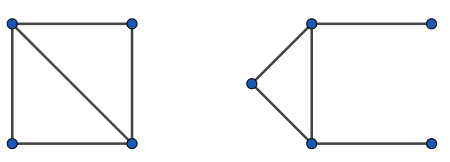
\includegraphics[width=.5\linewidth]{counting-colorings.png}%\hspace*{1cm}
\end{center}
I am honestly kind of stumped on this one sorry.
\clearpage
  We say a permutation $\sigma$ of $[2n]$ \textit{has property $P$} if
  \begin{equation*}
    |\sigma(i) - \sigma(i + 1)| = n
  \end{equation*}
  for some $i \in [2n]$ (in this problem, addition is modulo $2n$, so $\sigma(2n + 1)$ is defined to be $\sigma(1)$).  For example, the following permutation of $[6]$ has property $P$
  \begin{align*}
    1&&2&&3&&4&&5&&6\\%
    \downarrow&&\downarrow&&\downarrow&&\downarrow&&\downarrow&&\downarrow\\%
    2&&5&&4&&1&&2&&3
  \end{align*}
  because $\sigma(2) - \sigma(1) = 3$.  
\begin{problem}
  Prove that, for each $n \in \mathbb N$, there are more permutations with property $P$ than without it.
  \textit{Hint: Use the Inclusion-Exclusion Principle.  For each $i \in [2n]$, consider the set $A_i$ of permutations $\sigma$ satisfying $|\sigma(i) - \sigma(i + 1)| = n$, and show that $|A_i| = 2n(2n - 2)!$ and $A_i \cap A_{i+1} = \varnothing$ for all $i \in [2n]$.}
\end{problem}
\begin{proof}
    Let $A_k$ be the set of permutations with $k$ and $k + n$ in neighboring positions as $|\sigma(i) - \sigma (i + 1)| = |k - k + n| = |k + n - k| = n$ as per the problem definition. Let $A$ be the set of permutations with property $P$, so that $A$ is the union of the $A_k$. Then we have that $|A| = \sum_{k}|A_k| - \sum_{k < l} |A_k||A_l| + \sum_{k < l < m} |A_k||A_l||A_m| - ...$, this is an alternating sequence with decreasing terms, implying that $|A| \geq \sum_{k}|A_k| - \sum_{k < l}|A_k||A_l|.$ Then we have that $|A_k| = 2(2n-1)!$ since we have two orders for $k$ and $k + n$ and then $(2n - 1)!$ ways of arranging the $2n-1$ items if we treat $k$ and $k + n$ as a single item. Similarly $|A_k||A_l| = 4(2n - 2)!$ so we have that $|A| \geq 2n^2(2n-2)! > (2n)!/2$. This shows then that there are more permuations with the property $P$ than without the property $P$ as desired.
\end{proof}
\clearpage
\begin{problem}
  Let $\cF = \{A_1, \dots A_m\}$ be a family of subsets of a finite set $X$.  For $x \in X$, let $d_\cF(x)$ be the number of members of $\cF$ containing $x$.  Prove that
  \begin{equation*}
    \sum_{i=1}^m\sum_{j=1}^m |A_i \cap A_j| = \sum_{x \in X}d_\cF(x)^2.
  \end{equation*}
\end{problem}
\begin{proof}
    Let assumptions be as in the problem statement. Define a function $d_{\cF}(x)$ be the number of elements of $\cF$ containing $x$ for any $x\in X$. Then we have that $\sum_{i, j = 1}^m |A_i \cap A_j| = \sum_{i = j}^m|A_i \cap A_j| + \sum_{i \neq j}^m |A_i \cap A_j|$ when $x \in A_i$ but $x \not\in A_j$ then $A_i \cap A_j = \emptyset$ but when $A_i, A_j \subseteq X \Rightarrow x\in X, x\in A_i, A_j$ except for when $A_i, A_j = \emptyset.$ then we know that $\sum_{i, j = 1}^m |A_i \cap A_j| = \sum_{i, j = 1}^m |A_i| + \sum_{i, j = 1}^m |A_i \cap A_j| = \sum_{j = 1}^m |A_i \cap A_j|$ (for fixed $i$ in the last sum) will have $m^2$ possibilities as $A_j$ will have $m$ possibilities and $A_i$ will also have $m$ possibilities. Therefore, $\sum_{i = 1}^m\sum_{j = 1}^m |A_i \cap A_j| = \sum_{x\in X} d_{\cF}(x)^2$ as desired.
\end{proof}
\end{document}

%%% Local Variables:
%%% mode: latex
%%% TeX-master: t
%%% End:
